% =====================================================================
% Final Presentation — Parameter Golf
% CS586: Big Data Analytics — Spring 2026
% Compile: pdflatex presentation.tex
% Theme: metropolis. If unavailable, swap for \usetheme{Madrid}.
% =====================================================================
\documentclass[aspectratio=169,10pt]{beamer}

\usetheme{metropolis}
\usepackage{graphicx}
\usepackage{booktabs}
\usepackage{xcolor}
\usepackage{tikz}
\usepackage{hyperref}
\usepackage{appendixnumberbeamer}

\usetikzlibrary{positioning, arrows.meta, shapes.geometric, calc, fit, backgrounds}

\graphicspath{{figures/}}

% ---------- Color palette ----------
\definecolor{primary}{HTML}{1f4e79}
\definecolor{accent}{HTML}{c0392b}
\definecolor{ok}{HTML}{1e8449}
\definecolor{warn}{HTML}{b9770e}
\definecolor{soft}{HTML}{f4f1ec}
\definecolor{ink}{HTML}{1a1a1a}

\setbeamercolor{normal text}{fg=ink, bg=white}
\setbeamercolor{alerted text}{fg=accent}
\setbeamercolor{example text}{fg=ok}
\setbeamercolor{progress bar}{fg=primary, bg=primary!20}
\setbeamercolor{title separator}{fg=primary}
\setbeamercolor{frametitle}{bg=primary, fg=white}

\metroset{titleformat=smallcaps, sectionpage=progressbar, numbering=fraction}

% ---------- Helper macros ----------
\newcommand{\good}[1]{\textcolor{ok}{\textbf{#1}}}
\newcommand{\bad}[1]{\textcolor{accent}{\textbf{#1}}}
\newcommand{\hil}[1]{\textcolor{primary}{\textbf{#1}}}
\newcommand{\bpb}{\,bpb}

% =====================================================================
% Title
% =====================================================================
\title{Architecture and Training Design \\ Under a Hard Parameter Budget}
\subtitle{A Controlled Ablation Study at 16~MB}
\author{Shyam Patadia \\ \texttt{spatadia@wpi.edu}}
\institute{Worcester Polytechnic Institute \\ CS586: Big Data Analytics}
\date{Spring 2026 \\[0.4em] \footnotesize \href{https://github.com/shyampatadia/parameter-golf}{github.com/shyampatadia/parameter-golf}}

\begin{document}

% --------------------------------------------------------------- 1
\maketitle

% =====================================================================
% ACT I — THE QUESTION
% =====================================================================

% --------------------------------------------------------------- 2
\begin{frame}{Can a language model fit in 16~MB?}
\centering
\Large
That's smaller than \emph{a single MP3 song}.\\[0.4em]
Smaller than a typical PowerPoint deck.\\[0.4em]
\hil{1{,}000$\times$ smaller than GPT-2.}\\[1.2em]

\normalsize
OpenAI's \emph{Parameter Golf} challenge sets exactly this constraint:
\begin{itemize}
    \item Train a model from scratch.
    \item Ship weights $+$ training code in $\leq$ \hil{16{,}000{,}000~bytes}.
    \item Score: how well it predicts unseen English text.
\end{itemize}

\vspace{0.6em}
\textbf{Reference to beat:} \hil{1.2244\bpb} (the challenge's published INT8 baseline).
\end{frame}

% --------------------------------------------------------------- 3
\begin{frame}{First, what does ``score'' mean? -- bits per byte}
\begin{columns}[T,onlytextwidth]
\column{0.55\textwidth}
\textbf{bpb} = how many \emph{bits} the model needs to \emph{guess each byte} of unseen text.\\[0.5em]

It's the same as a compression ratio: a good model compresses text;
a bad model wastes bits on wrong guesses.

\vspace{0.7em}
\textbf{The scale:}
\begin{itemize}\setlength{\itemsep}{2pt}
  \item \bad{8.0\bpb} -- random guessing over all 256 byte values (no model)
  \item \warn{$\sim$4.5\bpb} -- guess letter frequency only
  \item \hil{1.2244\bpb} -- the challenge baseline
  \item \good{$\sim$1.0\bpb} -- frontier large LMs (GPT-4 class)
  \item \textbf{0\bpb} -- a perfect oracle
\end{itemize}

\vspace{0.6em}
\textcolor{accent}{\textbf{Lower is better.}} \\
Every 0.01\bpb is a real, measurable quality difference.

\column{0.45\textwidth}
\centering
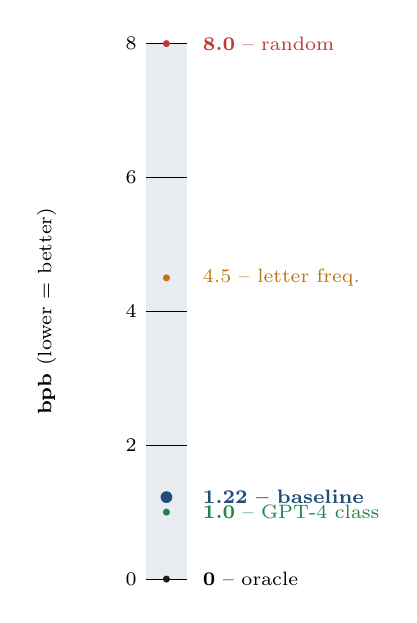
\begin{tikzpicture}[scale=0.85, every node/.style={font=\scriptsize}]
% Vertical scale bar
\fill[primary!10] (0,0) rectangle (0.6, 8);
\foreach \y/\lab in {0/0, 2/2, 4/4, 6/6, 8/8} {
  \draw (0,\y) -- (0.6,\y);
  \node[left] at (0,\y) {\lab};
}
\node[rotate=90, above] at (-1.2, 4) {\textbf{bpb} (lower = better)};

% Annotations on the right
\node[right, accent] at (0.7, 8.0)  {\bad{8.0} -- random};
\node[right, warn]   at (0.7, 4.5)  {\warn{4.5} -- letter freq.};
\node[right, primary, font=\scriptsize\bfseries] at (0.7, 1.2244) {\hil{1.22} -- baseline};
\node[right, ok]     at (0.7, 1.0)  {\good{1.0} -- GPT-4 class};
\node[right]         at (0.7, 0.0)  {\textbf{0} -- oracle};

% Markers
\fill[accent]  (0.3, 8.0)    circle (1.5pt);
\fill[warn]    (0.3, 4.5)    circle (1.5pt);
\fill[primary] (0.3, 1.2244) circle (2.5pt);
\fill[ok]      (0.3, 1.0)    circle (1.5pt);
\fill[ink]     (0.3, 0.0)    circle (1.5pt);
\end{tikzpicture}
\end{columns}
\end{frame}

% --------------------------------------------------------------- 4
\begin{frame}{How does a model become a 16~MB artifact?}
\centering
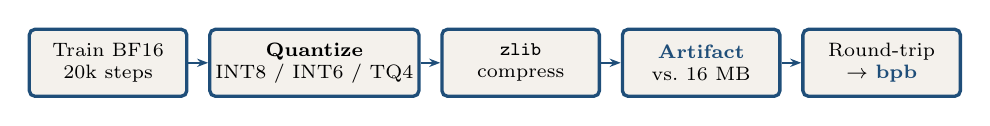
\begin{tikzpicture}[
  every node/.style={font=\scriptsize, align=center},
  box/.style={rectangle, rounded corners=2pt, draw=primary, very thick,
              fill=soft, minimum width=2.0cm, minimum height=0.85cm,
              inner sep=2pt},
  arr/.style={-{Stealth[length=4pt]}, primary, thick}
]
\node[box] (train)  {Train BF16 \\ 20k steps};
\node[box, right=0.25cm of train] (quant) {\textbf{Quantize}\\ INT8 / INT6 / TQ4};
\node[box, right=0.25cm of quant] (zlib)  {\texttt{zlib} \\ compress};
\node[box, right=0.25cm of zlib]  (size)  {\hil{Artifact}\\ vs.\ 16~MB};
\node[box, right=0.25cm of size]  (eval)  {Round-trip\\ $\rightarrow$ \hil{bpb}};

\draw[arr] (train) -- (quant);
\draw[arr] (quant) -- (zlib);
\draw[arr] (zlib)  -- (size);
\draw[arr] (size)  -- (eval);
\end{tikzpicture}

\vspace{0.9em}
\small This study has \hil{three levers} to push:
\begin{columns}[T,onlytextwidth]
\column{0.32\textwidth}\centering
\textbf{Architecture}\\ {\scriptsize depth, width, attention}
\column{0.32\textwidth}\centering
\textbf{Quantizer}\\ {\scriptsize INT8, INT6, TurboQuant-INT4}
\column{0.32\textwidth}\centering
\textbf{Recipe}\\ {\scriptsize optimizer, schedule, init}
\end{columns}

\vspace{0.7em}
\small \textbf{Method:} \emph{vary one lever at a time} -- 47 of 48 knobs held fixed.\\
\hil{46 controlled 20k-step runs} on FineWeb.
\end{frame}

% =====================================================================
% ACT II — PULLING THE LEVERS
% =====================================================================

% --------------------------------------------------------------- 5
\begin{frame}{Lever \#1: precision -- the highest-leverage knob}
\textbf{Intuition:} at 16~MB, INT8 fits $\sim$8M params, INT6 fits $\sim$11M.\\
Lower precision $=$ more capacity. \emph{Should} be a free win.

\vspace{0.5em}
\begin{columns}[T,onlytextwidth]
\column{0.55\textwidth}
\centering
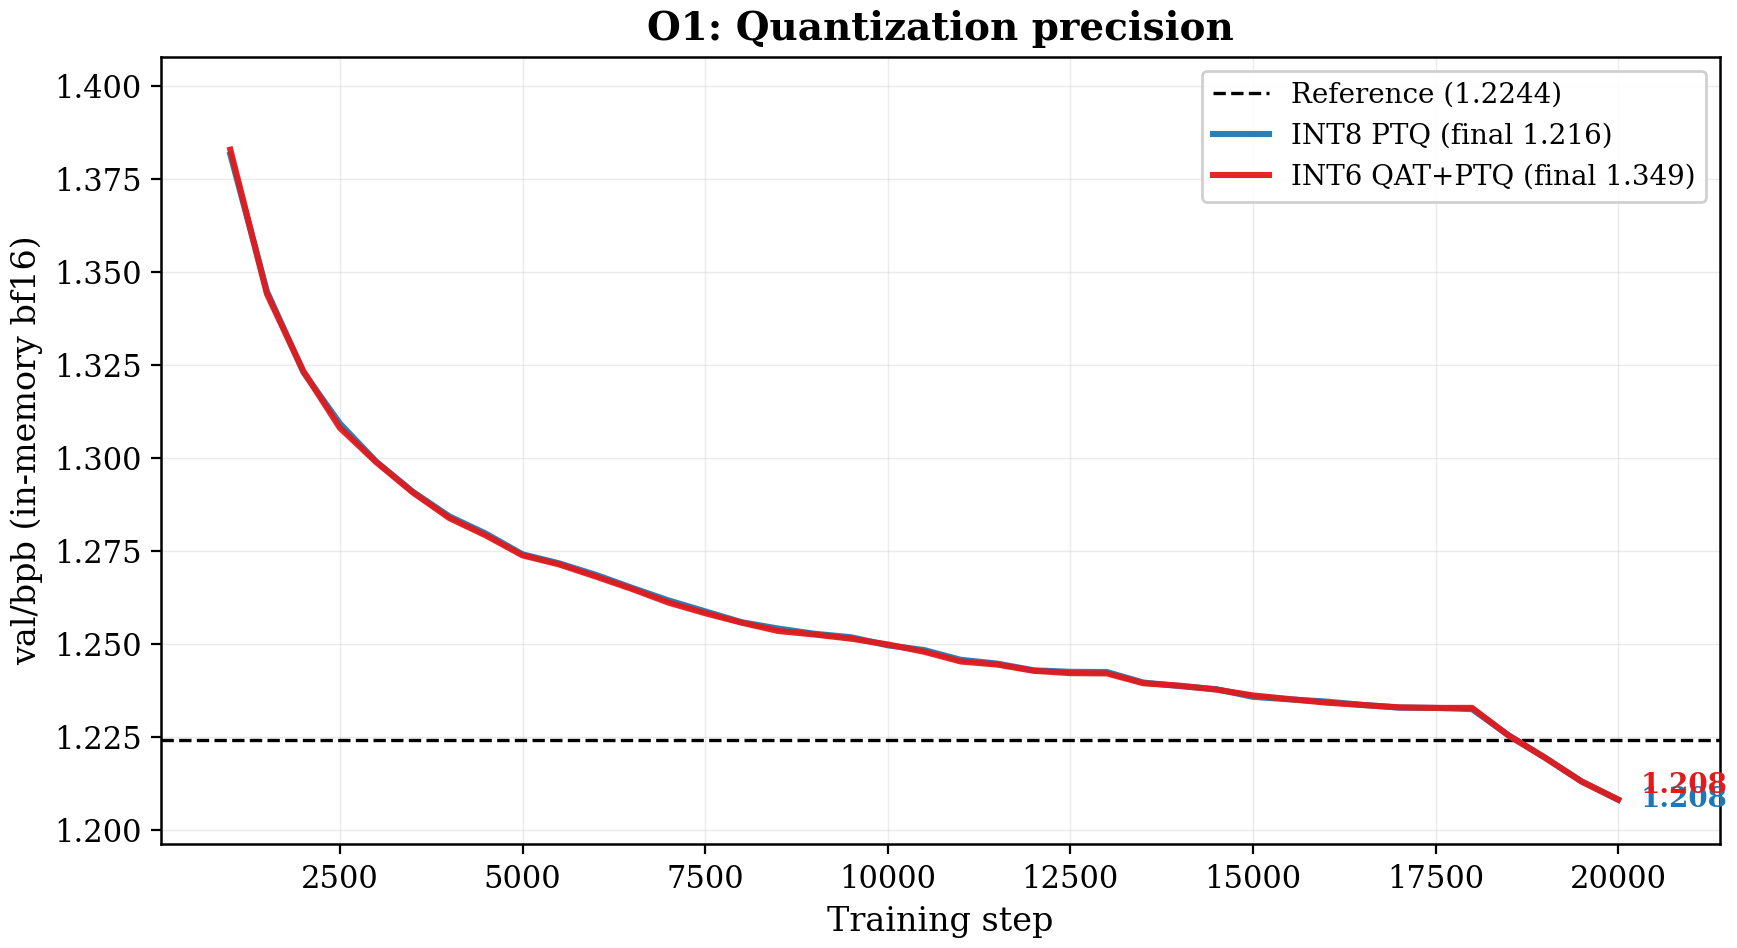
\includegraphics[width=\linewidth]{curves_o1_quant.pdf}

\column{0.45\textwidth}
\textbf{Training-time:} INT6 and INT8 reach the \emph{same} loss.\\[0.4em]
\textbf{After zlib roundtrip:}
\begin{itemize}
  \item INT8: \good{1.216\bpb} ($\Delta_q = 0.008$)
  \item INT6: \bad{1.349\bpb} ($\Delta_q = 0.141$)
\end{itemize}

\vspace{0.4em}
\textcolor{accent}{\textbf{Surprise.}} Quantization-aware training matches the
loss \emph{in memory}, but uniform 6-bit scales can't represent the trained
weights. \\[0.4em]

\hil{Lesson: more bits to spend $\neq$ more capacity if you can't read them back.}
\end{columns}
\end{frame}

% --------------------------------------------------------------- 6
\begin{frame}{Levers \#2--4: position, optimizer, factorizations}
\begin{columns}[T,onlytextwidth]
\column{0.5\textwidth}
\centering
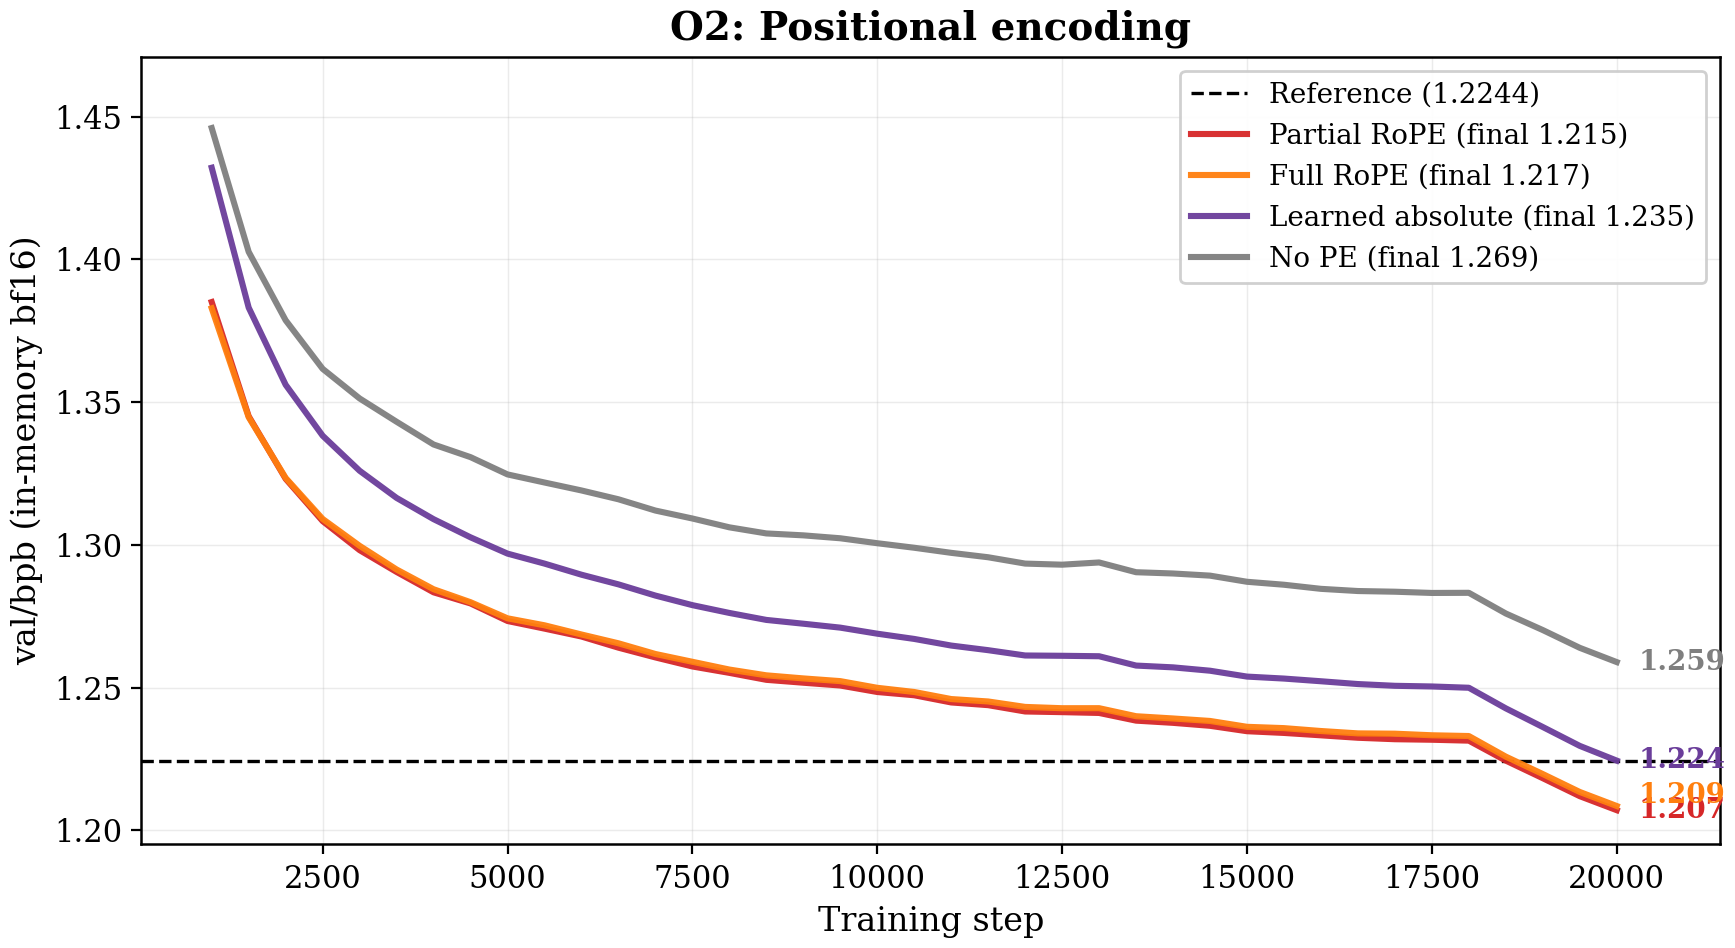
\includegraphics[width=\linewidth]{curves_o2_posenc.pdf}\\
{\scriptsize \textbf{Position:} Partial RoPE \good{1.215} -- best in-budget.\\
The \emph{form} of the prior is second-order; \emph{having} one is first-order.}

\column{0.5\textwidth}
\centering
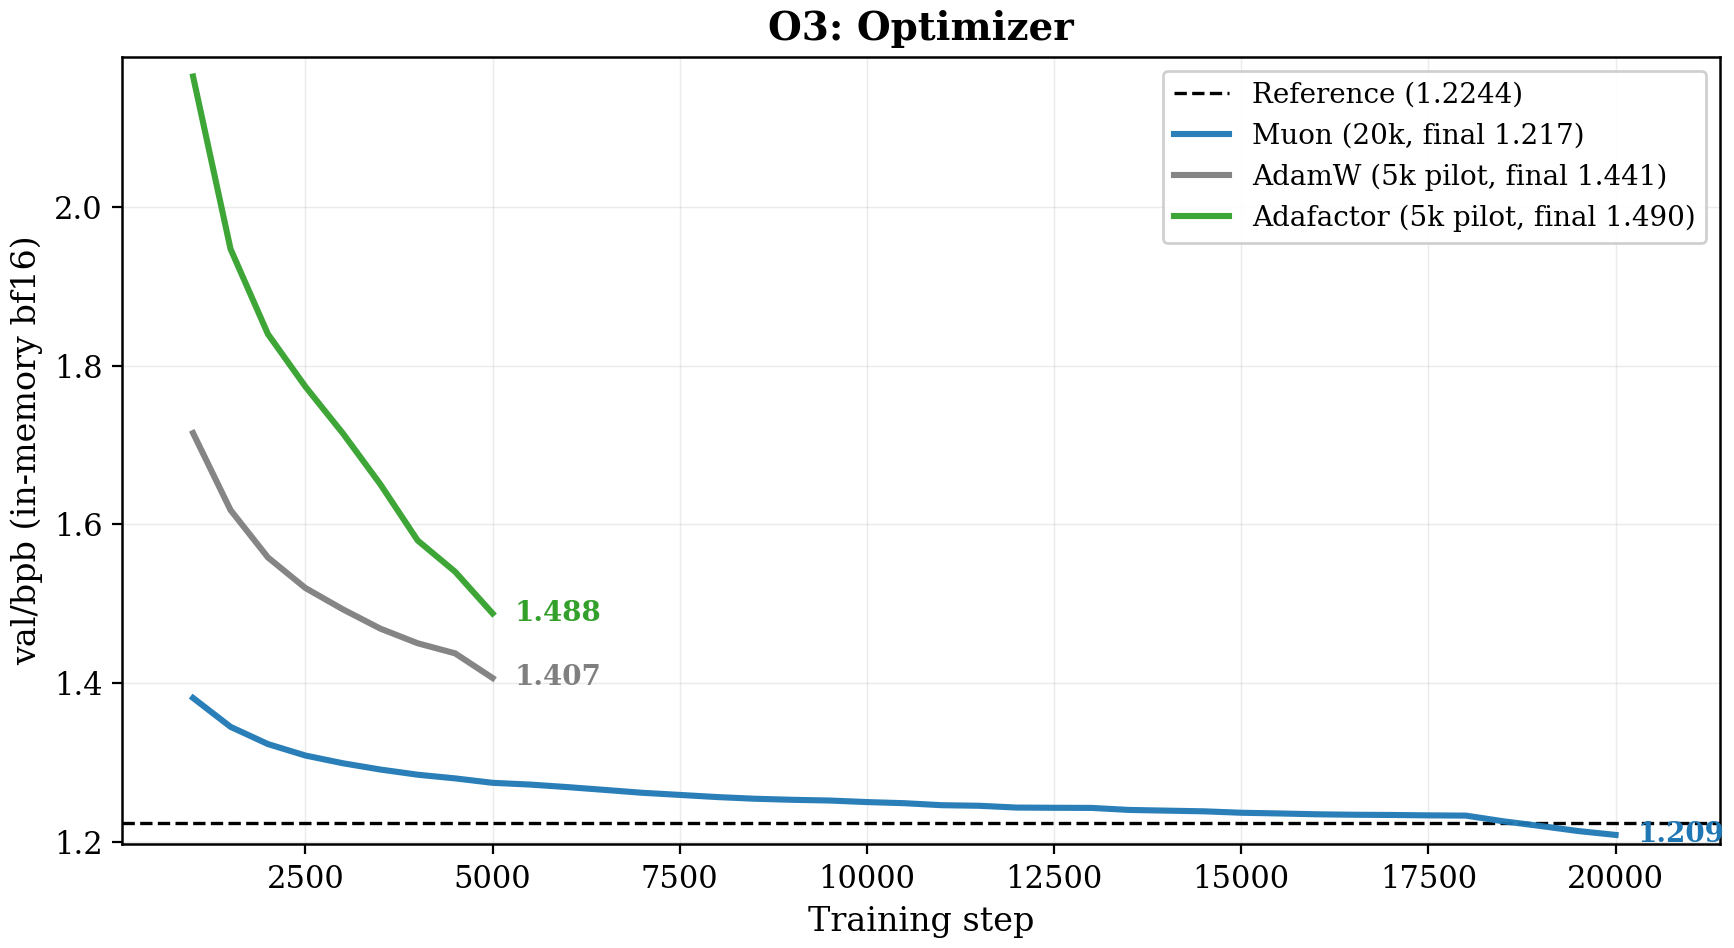
\includegraphics[width=\linewidth]{curves_o3_optim.pdf}\\
{\scriptsize \textbf{Optimizer:} Muon \good{1.217} $\ll$ AdamW (1.44), Adafactor (1.49). \\
\emph{Load-bearing -- not a tunable.}}
\end{columns}

\vspace{0.4em}
\hrule
\vspace{0.3em}
\textbf{What about clever weight factorizations?} (low-rank, block-diagonal, random projection)\\
$\rightarrow$ all land at \bad{1.30--1.40\bpb}. \hil{Falsified} as a capacity lever at this scale.

\end{frame}

% =====================================================================
% ACT III — THE PUZZLE AND THE RESOLUTION
% =====================================================================

% --------------------------------------------------------------- 7
\begin{frame}{Now stack the winners -- and watch them \emph{cancel out}}
\textbf{The natural next step:} combine everything that worked.\\
Partial RoPE (best position) $+$ INT6 (most bits) $+$ 11 layers $+$ MLP$=$3.

\vspace{0.6em}
\centering
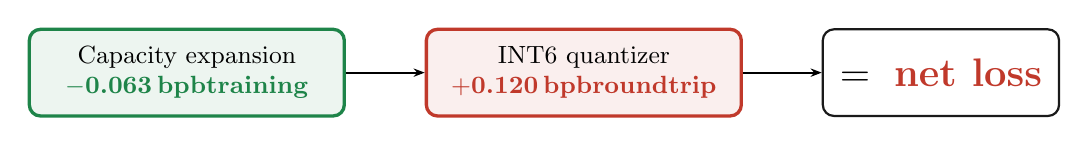
\begin{tikzpicture}[every node/.style={font=\small, align=center}]
\node[draw=ok, very thick, rounded corners, fill=ok!8,
      minimum width=4.0cm, minimum height=1.1cm] (a)
      {Capacity expansion \\ \good{$-$0.063\bpb training}};
\node[draw=accent, very thick, rounded corners, fill=accent!8,
      minimum width=4.0cm, minimum height=1.1cm, right=1.0cm of a] (b)
      {INT6 quantizer \\ \bad{$+$0.120\bpb roundtrip}};
\node[draw=ink, thick, rounded corners,
      minimum width=3.0cm, minimum height=1.1cm, right=1.0cm of b] (c)
      {\Large $=$ \;\bad{net loss}};

\draw[-{Stealth[length=4pt]}, thick] (a) -- (b);
\draw[-{Stealth[length=4pt]}, thick] (b) -- (c);
\end{tikzpicture}

\vspace{0.7em}
Training loss \good{1.1614\bpb} -- best ever.\\
Final loss \bad{1.2816\bpb} -- worse than baseline.

\vspace{0.7em}
\hil{Which lever is paying the bill -- the capacity, or the quantizer?}
\end{frame}

% --------------------------------------------------------------- 8
\begin{frame}{The decisive experiment: change one variable at a time}
Two follow-ups, each isolating \emph{one} side of the trade:

\begin{columns}[T,onlytextwidth]
\column{0.55\textwidth}
\centering
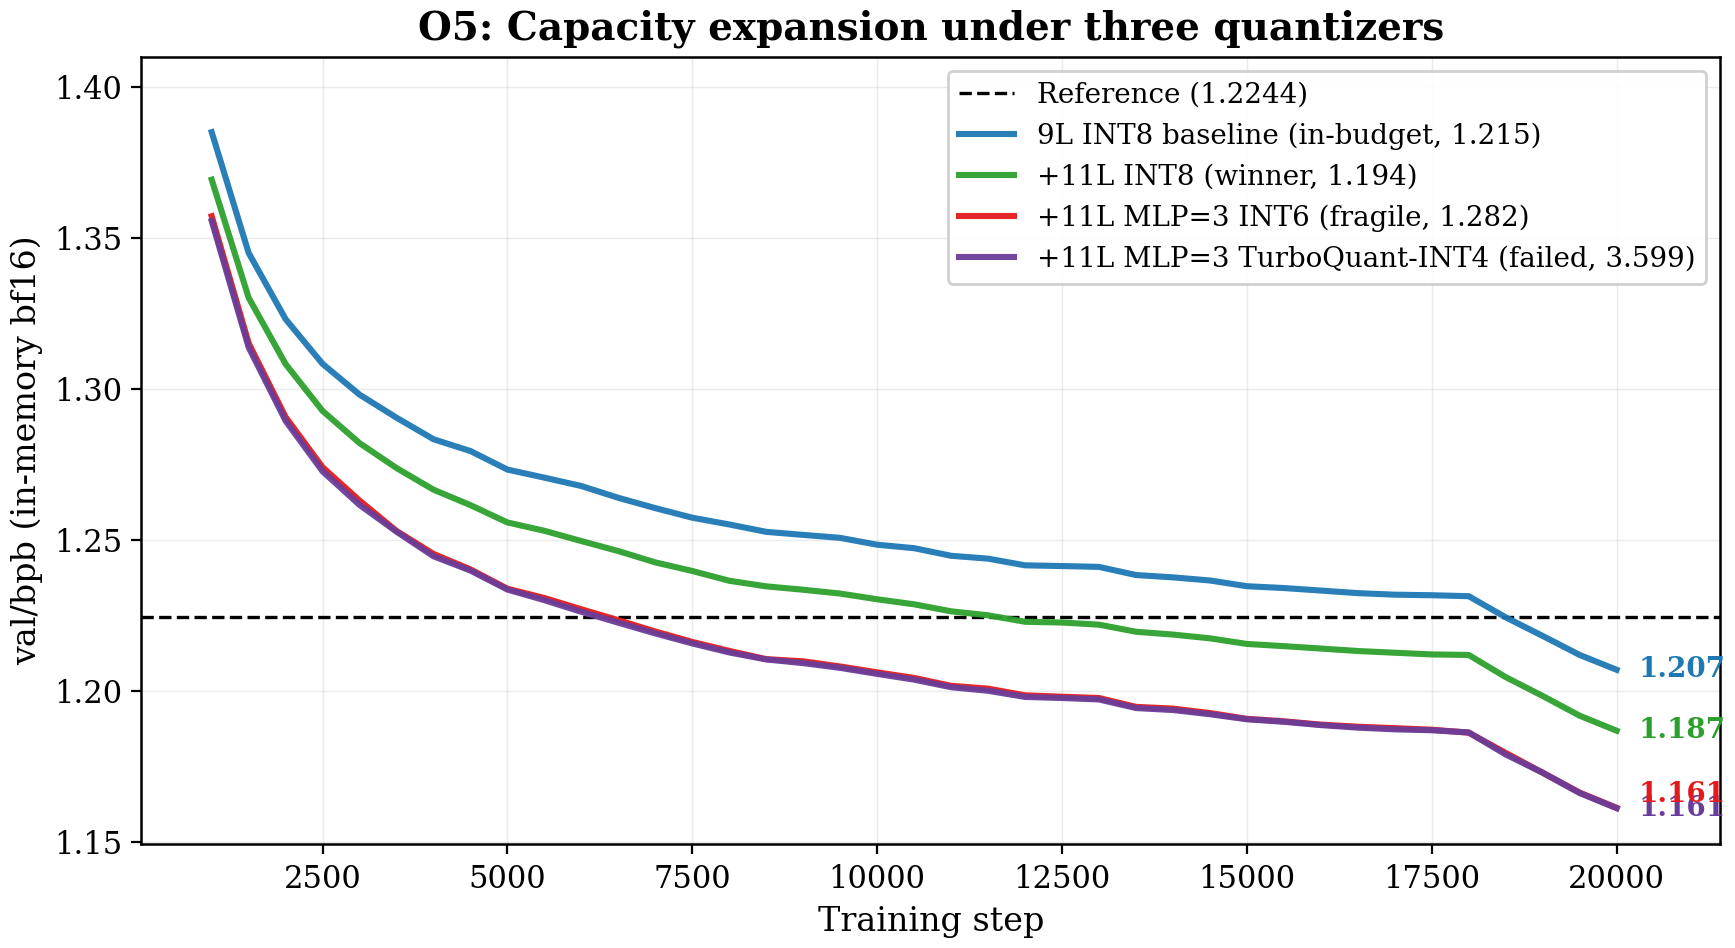
\includegraphics[width=\linewidth]{curves_o5_resolved.pdf}

\column{0.45\textwidth}
\textbf{(a) Same arch, swap quantizer:}\\
TurboQuant-INT4 (random rotation $+$ Lloyd--Max).\\
$\rightarrow$ \bad{3.60\bpb} final. Catastrophic.

\vspace{0.6em}
\textbf{(b) Same quantizer, ease arch:}\\
INT8 $+$ 11~layers $+$ MLP$=$2.\\
$\rightarrow$ \good{1.194\bpb}, $-$0.030 below reference.

\vspace{0.7em}
\hil{Verdict: the quantizer was paying the bill.}\\
The architecture lever works -- as long as you don't crush precision to fund it.
\end{columns}
\end{frame}

% --------------------------------------------------------------- 9
\begin{frame}{Three more levers we pushed (gains we banked + nulls we report)}
\small
\begin{columns}[T,onlytextwidth]
\column{0.5\textwidth}
\textbf{O6 -- Multi-Query Attention.}\\
1 KV head $\rightarrow$ free parameters $\rightarrow$ 12 layers fit.\\
\good{1.198\bpb} at 19.56~MB.\\[0.3em]
\centering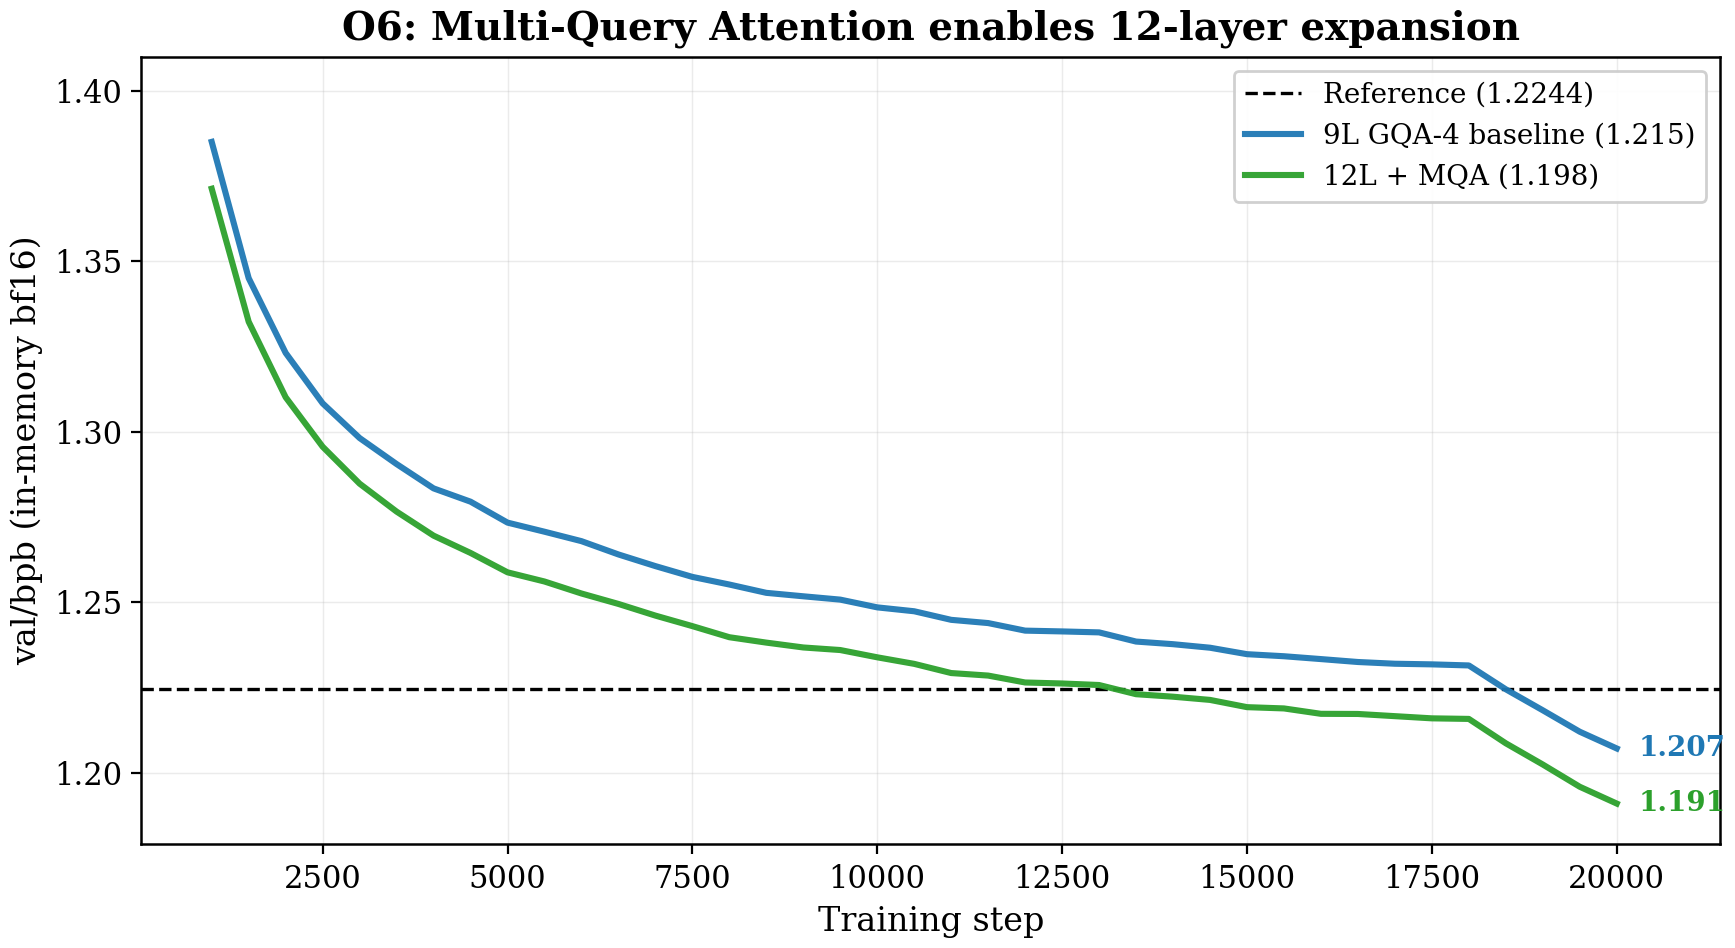
\includegraphics[width=0.95\linewidth]{curves_o6_mqa.pdf}

\column{0.48\textwidth}
\textbf{O7 -- QK-gain initialization.}\\
$g_q^{(0)} \in \{1.5, 3.0, 5.0\}$. Spread \alert{0.002\bpb}. \\
\hil{Null effect.} Learned $g_q$ converges regardless.\\[0.6em]

\textbf{O8 -- LR / warmup sweep ($3{\times}3$).}\\
Spread \alert{0.0019\bpb}. \\
\hil{Null effect.} Default recipe is at the optimum.\\[0.6em]

\textbf{O9 -- Eval protocol.}\\
Same weights; sliding-window stride-256 scores \hil{1.160\bpb}.\\
\textit{Apples-to-apples comparison requires non-overlapping windows.}
\end{columns}

\vspace{0.5em}
\hil{Three nulls are findings too} -- they constrain the design space and save future work.
\end{frame}

% =====================================================================
% ACT IV — THE BIG PICTURE
% =====================================================================

% --------------------------------------------------------------- 10
\begin{frame}{The headline: 16~MB is an \emph{elbow}, not a wall}
\centering
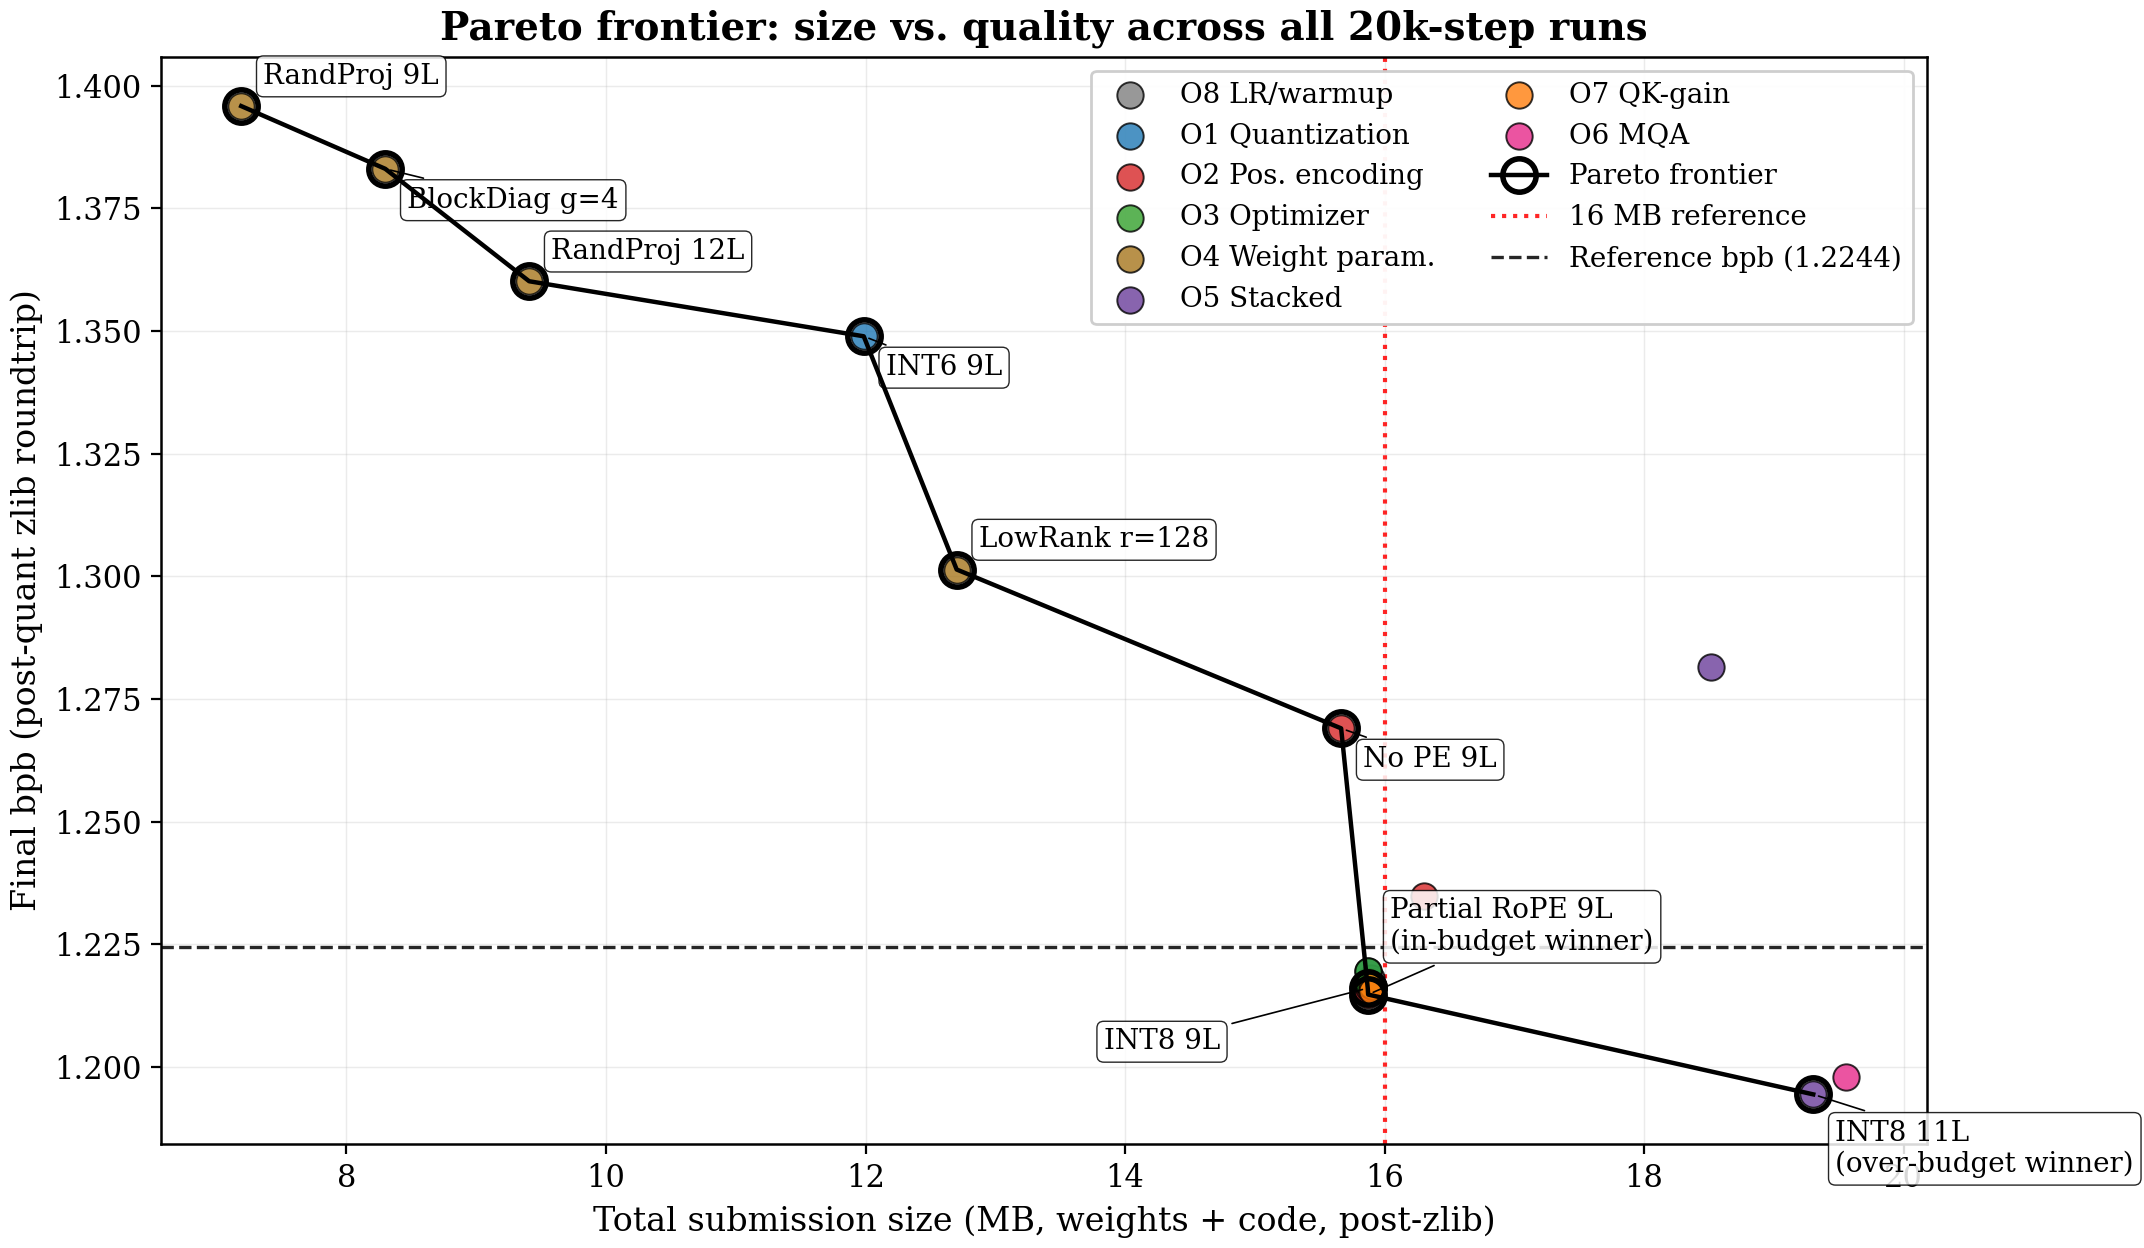
\includegraphics[width=0.92\linewidth]{pareto_frontier.pdf}

\vspace{-0.3em}
{\small Below 15.9~MB: every MB saved costs $\sim$0.02\bpb (steep).\\
Above 15.9~MB: marginal gains flatten. \\
\good{In-budget winner 1.215\bpb at 15.87~MB} \;\;|\;\; \good{over-budget winner 1.194\bpb at 19.30~MB}.}
\end{frame}

% --------------------------------------------------------------- 11
\begin{frame}{Are these numbers real, or seed luck?}
\begin{columns}[T,onlytextwidth]
\column{0.55\textwidth}
\centering
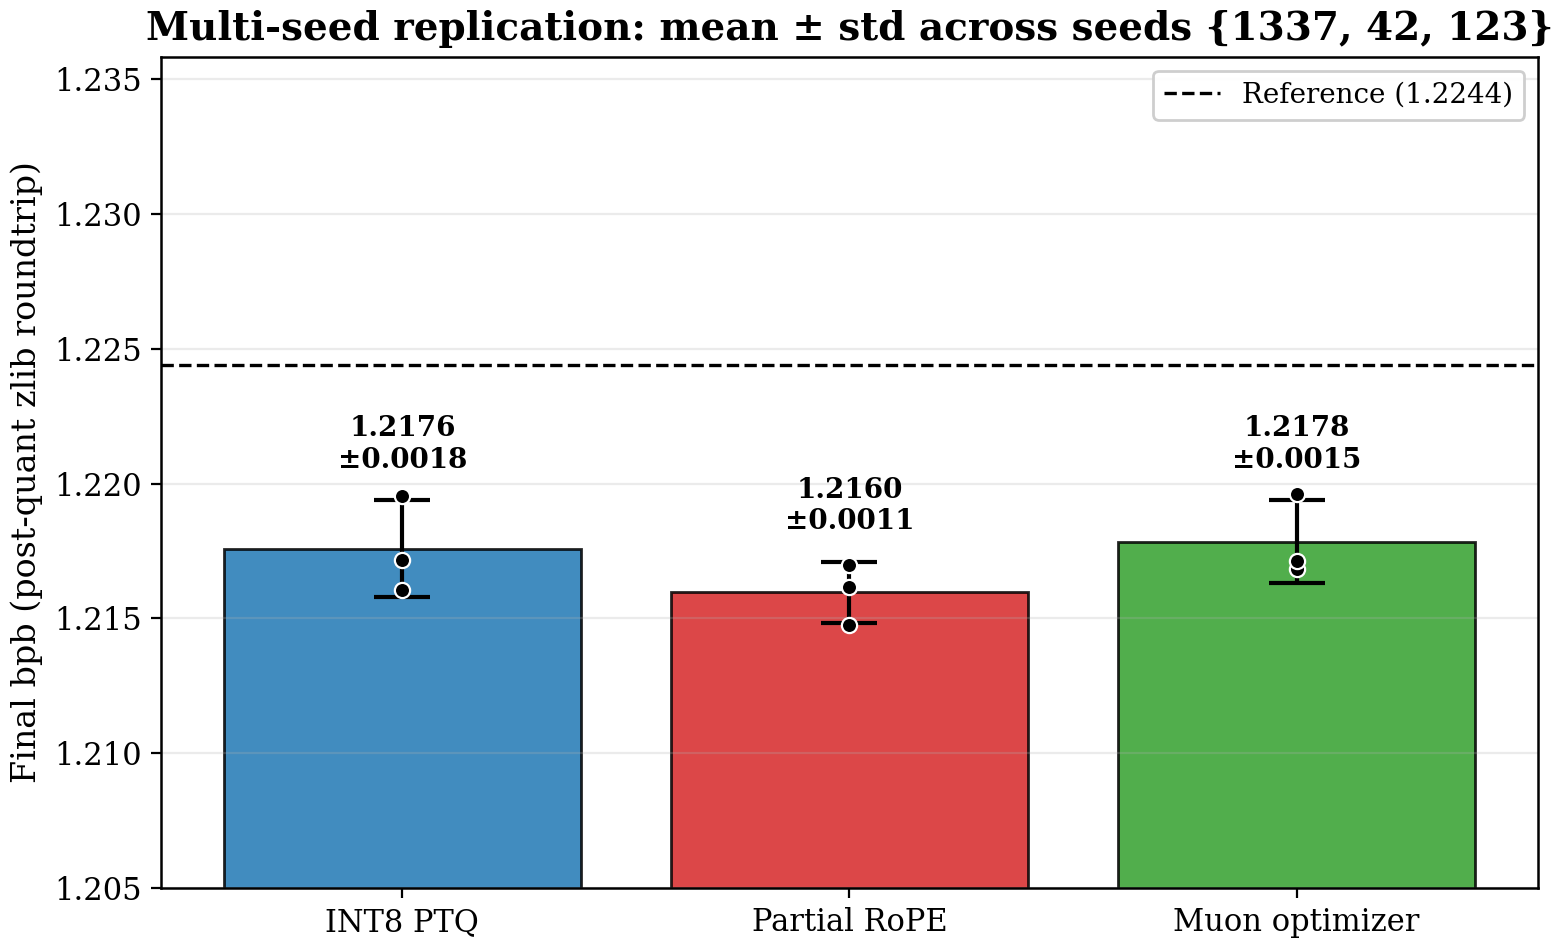
\includegraphics[width=\linewidth]{multiseed_bars.pdf}

\column{0.45\textwidth}
We re-ran the three surviving in-budget axes at seeds $\{1337, 42, 123\}$:
\begin{itemize}\small
  \item INT8 PTQ: $\sigma = 0.0018$
  \item Partial RoPE: $\sigma = 0.0011$
  \item Muon: $\sigma = 0.0015$
\end{itemize}

\vspace{0.7em}
Per-axis effects ($\sim$0.05--0.20\bpb) are \\ \hil{$10$--$100\times$ larger
than seed noise.} \\[0.3em]
The single-seed claims hold up.
\end{columns}
\end{frame}

% --------------------------------------------------------------- 12
\begin{frame}{What we learned}
\begin{enumerate}\setlength{\itemsep}{4pt}
  \item \hil{Sub-INT8 weight quantization is fragile at this scale.}
        QAT does not save INT6. Random rotation does not save INT4.
        The quantizer, not the recipe, is the binding constraint.
  \item \hil{Capacity expansion is real -- but only INT8 carries it.}
        Same architecture: under INT6 it forfeits its gain;
        under INT8 it lands $-$0.030\bpb below reference.
  \item \hil{Inductive biases matter at the margin, not the headline.}
        Partial RoPE, MQA, depth all help by $\sim$0.01--0.02\bpb;
        none rivals the precision lever in effect size.
  \item \hil{The 16~MB ``constraint'' is a soft Pareto elbow.}
        $+3.3$~MB buys 0.020\bpb. Not a binary; a continuous trade.
  \item \hil{Three nulls reported as findings:}
        weight factorizations, QK-gain init, LR/warmup. \\
        Negative results constrain the design space.
\end{enumerate}
\end{frame}

% --------------------------------------------------------------- 13
\begin{frame}[standout]
Thank you.\\[0.5em]
{\normalsize Questions?}\\[1.2em]
{\footnotesize \texttt{spatadia@wpi.edu}\\
\href{https://github.com/shyampatadia/parameter-golf}{github.com/shyampatadia/parameter-golf}}
\end{frame}

\end{document}
